 %!TEX root = main.tex
\chapter{Discrimination and fidelity}

Many biochemical reactions happen at extreme fidelity: DNA replication in some organisms makes fewer than one mistake in $10^{10}$ bases copied.
Mutation rates vary greatly across organisms: the smaller the genome, the higher the mutation rate.
This anti-correlation is shown in schematically in Fig.~\ref{fig:mutation_rates}.
This fidelity relies on energetic discrimination of the correct and wrong base pairing.
The difference in interaction energies of the correct (Watson-Crick) and non-basepairing configuration, however, is only a few kT.
The fact that extremely high accuracies can be achieved is therefore remarkable.

\begin{figure}[tb]
	\centering
	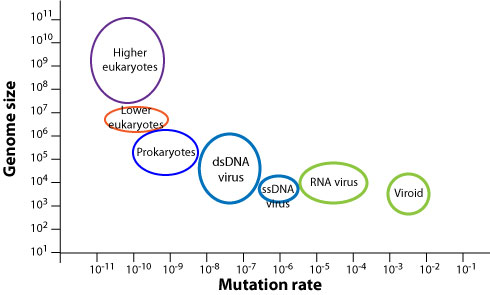
\includegraphics[width=\textwidth]{figures/mutation_rates.jpg}
	\caption{Mutation rates of various organisms vs their genome size.}
	\label{fig:mutation_rates}
\end{figure}

Why should we expect such an anti-correlation?
The probability that that the entire genome of length $L$ is copied faithfully is given by $\exp(-L\mu)$.
Hence as soon as the mutation rate is much larger than the inverse genome size, almost every new genome will contain mutations resulting in a gradual loss of functional sequence (a process known as Muller's ratchet).
If being accurate is costly in terms of energy amd/or time, you'd expect organisms to adjust fidelity to be just ``good enough''. Hence the scaling behavior of fidelity with genome length is plausible.

However, it is not at all a trivial question how high fidelity can be achieved given the small free energy differences associated with nucleotide mis-incorporation.
It was \citep{hopfield_kinetic_1974} and \citep{ninio_kinetic_1975} who first discussed mechanisms on how to achieve high fidelity in biochemical processes.
Fidelity is not only important in DNA replication, but also in translation, tRNA charging and signaling processes.

\section{Energies of discrimination}
Consider the following simple set of reactions
\begin{equation}
C + E \leftrightarrow CE \rightarrow \mathrm{correct}
\end{equation}
\begin{equation}
D + E \leftrightarrow DE \rightarrow \mathrm{wrong}
\end{equation}
The transition states CE and DE are populated according to the equilibrium constant of these reactions $K_C =k_C'/k_C$ and $K_D = k_D'/k_D$ where $k'_C$  and $k'_D$ are the on-rates and $k_C$, $k_D$ are the off-rates.
We assume that the product formation happens at the same rate $W$ for both the correct and incorrect transition state.
In other words, the discrimination between the wrong and the correct state happens in the formation of the transition state.
This is a sensible assumption in cases like polymerization reactions which can occur as long as the two entities are in place.
Furthermore, it is reasonable to assume that the on-rates $k_C'$ and $k_D'$ are similar since they are likely limited by diffusion.
The off-rates, on the other hand, are strongly dependent on the correct substrate match and this is where discrimination comes from.
Assuming that both on-rates are $k = k_C' = k_D'$, we can express the rate at which each product is formed as
\begin{equation}
W[Cc] = W\frac{k[C]}{k_C+W}
\end{equation}
\begin{equation}
W[Dc] = W\frac{k[D]}{k_D+W}
\end{equation}
and hence the ratio of correct to wrong product is
\begin{equation}
\frac{\mathrm{correct}}{\mathrm{wrong}} = \frac{[C]}{[D]}\frac{k_D+W}{k_C + W} \rightarrow \frac{[C]}{[D]}\frac{k_D}{k_C} =  \frac{[C]}{[D]}e^{-\Delta G/kT}
\end{equation}
Here the last two expressions assumed that the product formation rate $W$ is much smaller than the off-rates of the transition state.
The very last equality expressed the off-rate dependence in terms of the difference in free energy of the transition states and thereby defines the {\bf energy of discrimination}.
Hence in any off-rate dominated discrimination, the differences in free energy put an upper bound on the accuracy of the process.
However, the binding energy differences of incorrect nucleotide reactions are on the order of a few kT and while accuracy of DNA replication would seem to require energies of discrimination on the order of 20kT.
This conundrum is what kinetic proofreading resolves in an elegant way.

\section{Irreversible intermediate states and kinetic proof reading}
Kinetic proof reading requires additional steps in the pathway to final product, but at least one of these steps needs to be coupled to an additional energy consuming reaction that makes the pathway irreversible.
The need for such an additional step is seen as follows: A reaction that proceeds via two intermediate states $XE$ and $XE'$ can effectively be compressed into one
\begin{equation}
X + E \leftrightarrow XE \leftrightarrow  XE' \rightarrow \mathrm{product}
\end{equation}
\begin{equation}
X + c \leftrightarrow  XE' \rightarrow \mathrm{product}
\end{equation}
or put otherwise the second intermediate state is in equilibrium with the same discriminatory ratio as before.

If, however, the transition from $XE$ to $XE' $ is coupled to an irreversible reaction while $XE'$ can still decay into $X+E$, higher accuracy can be attained.
In this case, the state $XE'$ can only be reached via $XE$ which is already selected for the correct product by a factor $e^{-\Delta G/kT}$.
If the rates of decay of $XE'$ for C and D are again different by a factor $e^{-\Delta G/kT}$, the overall accurary of the process can be as high as $e^{-2\Delta G/kT}$.

The accuracy of a process can be increased exponentially by adding more and more intermediate states.

\subsection*{Interpretation of proof-reading as a delay}
The addition of an irreversible step essentially changes the distribution of times the product spends in the transition state.
While being in the transition state, the correct pair decays as $e^{-k_Ct}$ and the wrong product as $e^{-k_Dt}$ such that the ratio behaves as $e^{-(k_C-k_D)t}$.
In a one step reaction, the distribution of residence times in the transition state has a peak at $t=0$ and decays exponentially. In a two-step reaction, this distributions has a peak away from zero.
This can be seen as follows.
Consider the a transition state $XE$ the moment it is formed. The probability $p(t)$ of still being intact is given by
\begin{equation}
\frac{dp}{dt} = - (k_X + W)p(t) \quad \Rightarrow\quad p(t) = e^{-(k_X+W)t}
\end{equation}
where $W$ is the rate at which the second intermediate is formed.
The probability $q(t)$ of being in the second intermediate is then
\begin{equation}
\frac{dq}{dt} = Wp(t) - Vq(t) = We^{-(k_X+W)t} - Vq(t)
\end{equation}
The latter has the solution
\begin{equation}
q(t) = We^{-Vt}\int_0^t e^{(V-W-k_X)t'} dt' = \frac{We^{-Vt}}{W+k_X-V}\left[1-e^{-(W+k_X - V)t}\right]
\end{equation}
While in a single step reaction the product starts being formed immediately, product formation starts gradually in a two step reaction.
This delay give the wrong intermediate complexes more time to break up and hence better discrimination.
